\section{Conclusion}
\label{sec:conclusion}

%In this laboratory assignment the objective of building an audio amplifier was achieved.
% The cost of the circuit was of $ 2102.508 MU$ and the merit $3.238$.
% 
%The results from both the theoretical analysis using octave and the circuit
%simulation using ngspice appear to roughly match, as we can see in the following figure and table:
%
%
%
%\begin{minipage}[c]{0.50\linewidth}
%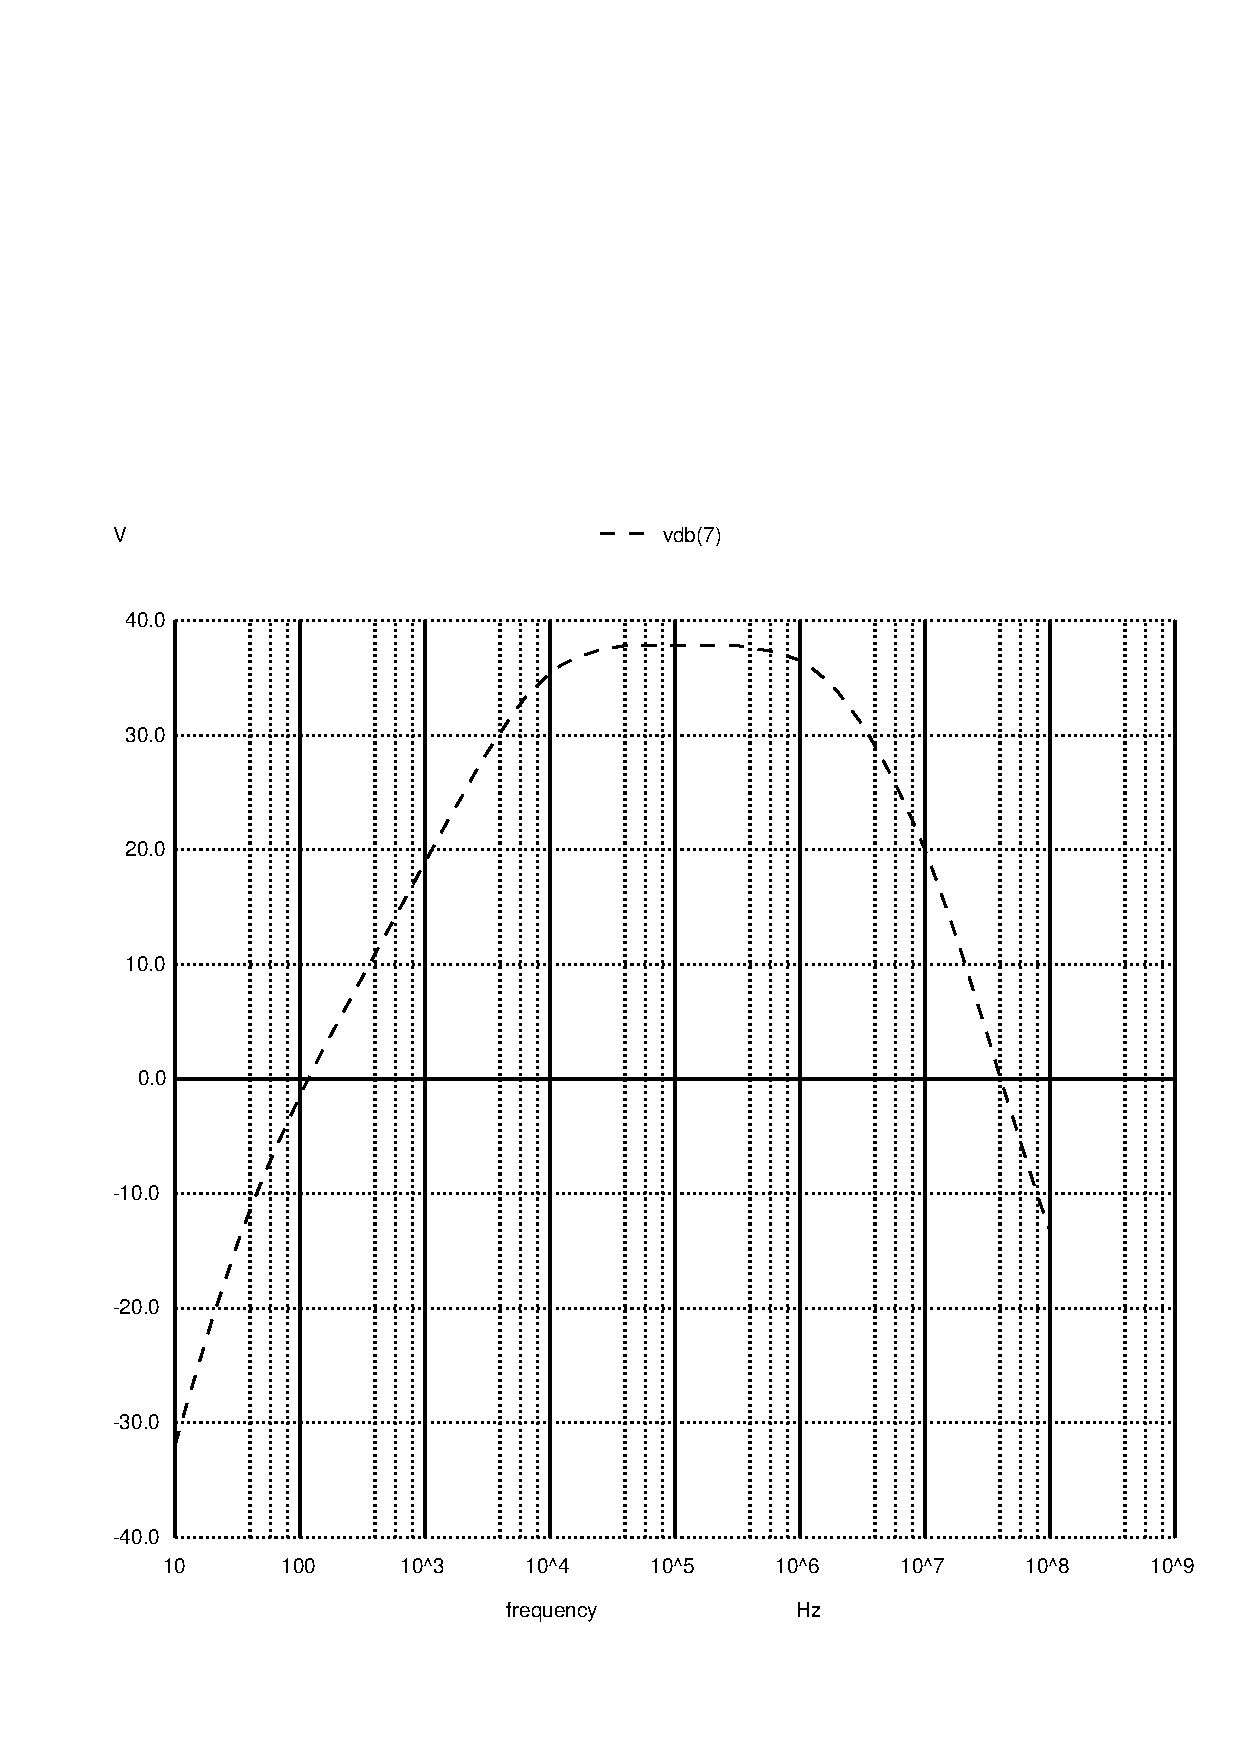
\includegraphics[width=1\linewidth]{../sim/vo2f.pdf}
%\end{minipage} % no space if you would like to put them side by side
%\hspace{1mm}
%\begin{minipage}[c]{0.50\linewidth}
%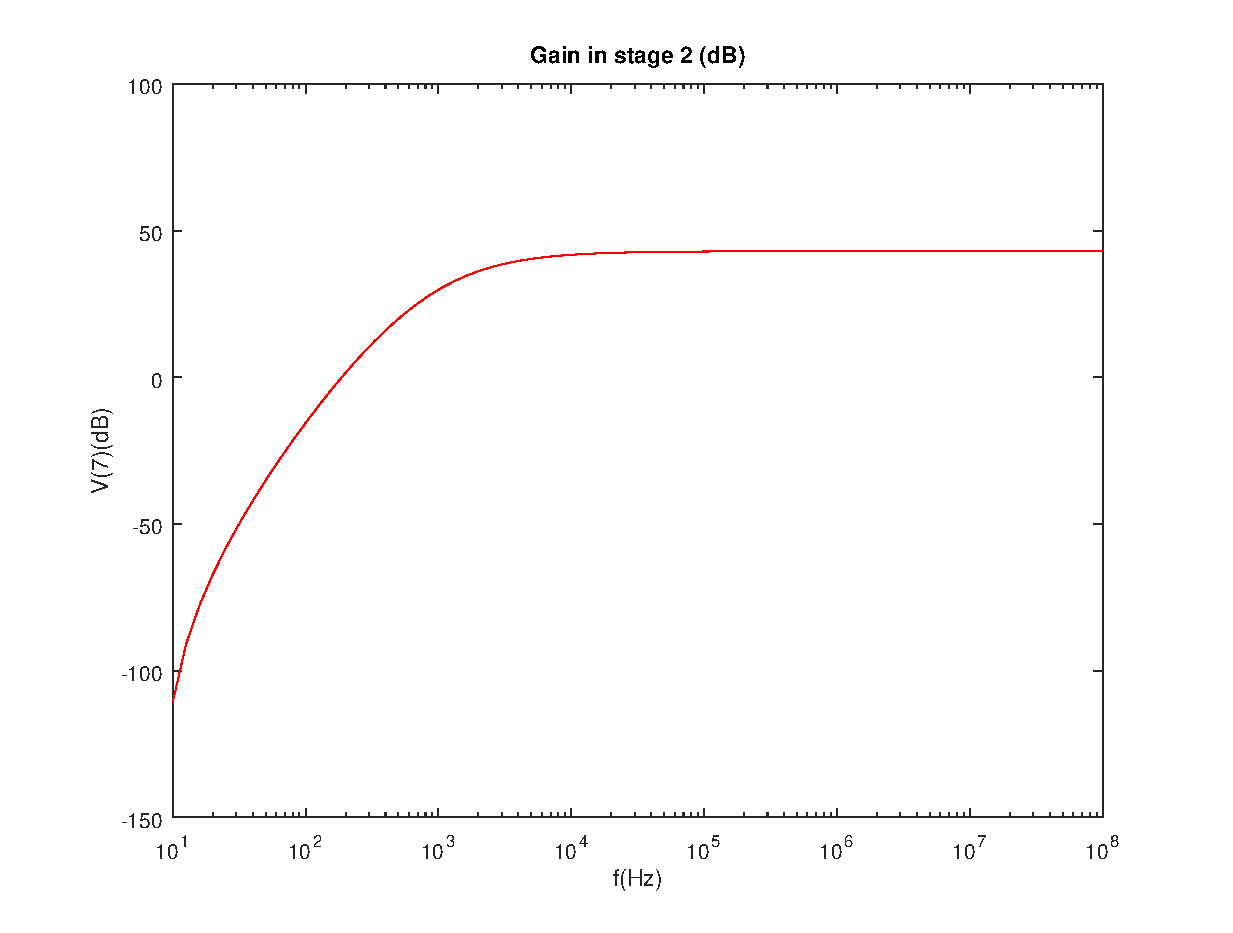
\includegraphics[width=1\linewidth]{vo2.eps}
%\end{minipage}
%
%We can see that the gain for the second stage is fairly different. The simulation has a drop at around $10^6$ Hz, while the theoretical model mantains steadily at around 45dB.
%
%Comparing all of the other values, we get the following table: 
%
%
%\begin{table}[H]
%\addtolength{\tabcolsep}{-4pt}
%\caption{Values of gain and input and output impedance for theoretical and simulation analysis}
%\vspace{-3mm}
%\begin{tabular}{|c|c|c|}
%\hline
% &	Mat &	Sim\\
%
%Zi1 &484.43 &	563.83 \\
%
%Zo1&886.28 	&-\\
%
%Zi2&	8598.9 	&-\\
%
%Zo2&	0.30217 &	10.07 \\
%
%Gain1&	48.392 dB	&-\\
%
%Gain2&	-0.0702 dB&-\\	
%
%GainT&	48.322 dB	&37.904 dB\\
%
%LowCOP&	5.48 kHz&	8.88 kHz\\
%
%BdWth	&-	&1.60 MHz\\
%
%Cost	&2102.508 MU&	2102.508 MU\\
%\hline
%\end{tabular}
%\label{tab:Comparison}
%\end{table}
%
%We can compare directly the input impendance for stage 1, Zi1: The theoretical model gives a lower value, about $86\%$ of the simulated one. Same goes for the output impedance, Zo2, where the theoretical analysis gives $\approx 0.3$, which is only around $3\%$ of what the simulation gives.
%
%\par
%We can conclude that there are various differences between the theoretical and simulation analysis. These can be attributed to the various aproximations
%made in the theoretical analysis, in the ideal transistor model for example, while the simulation uses a comparatively accurate spice model. The simulation therefore gives more credible values, closer to reality.
%